\documentclass[11pt, a4paper]{article}
\usepackage[a4paper,margin=1in,footskip=0.25in]{geometry}


% load package with some of the available options - you may not need this!
\usepackage[framed,autolinebreaks,useliterate]{mcode}

% for checklist
\usepackage{enumitem,amssymb}
\newlist{todolist}{itemize}{2}
\setlist[todolist]{label=$\square$}
\usepackage{pifont}
\newcommand{\cmark}{\ding{51}}%
\newcommand{\xmark}{\ding{55}}%
\newcommand{\done}{\rlap{$\square$}{\raisebox{2pt}{\large\hspace{1pt}\cmark}}%
\hspace{-2.5pt}}
\newcommand{\wontfix}{\rlap{$\square$}{\large\hspace{1pt}\xmark}}


% something NOT relevant to the usage of the package.
\usepackage{graphicx}
\usepackage{url,textcomp}
\setlength{\parindent}{0pt}
\setlength{\parskip}{18pt}
\title{ECTA Homework 4\\Multiobjective Optimization with the\\Non-dominated Sorting Genetic Algorithm II}
\author{\color{blue}Erick Kramer, Mihir Patil\\ \texttt{\color{blue}erick.romero@smail.inf.h-brs.de , mihir.patil@smail.inf.h-brs.de}}
% //////////////////////////////////////////////////

\begin{document}

\maketitle

%\begin{center}
%	\begin{minipage}{1\linewidth}
%		\begin{center}
%			\includegraphics[width=\textwidth]{xkcd}
%		\end{center}
%	\end{minipage}
%\end{center}

\newpage

\section{Assignment Description}
	\begin{enumerate}
		\item Implement the NSGA-II algorithm and apply it to a toy problem
			\begin{itemize}
			\item Bit string with length 20
			\item Maximize the number of leading zeros (zeros in a row at the front)
			\item Maximize the number of trailing ones (ones in a row at the back)
		\end{itemize}
		\item Show that your algorithm works by plotting the population at various stage of the algorithm
	\end{enumerate}

\section{Submission Instructions}
Follow along with the instructions in this PDF, filling in your own code, data, and observations as noted. Your own data should be inserted into the latex code of the PDF and recompiled. All code must be done in MATLAB.

To be perfectly clear we expect two submissions to LEA:
\begin{enumerate}
	\item 1 PDF (report) -- a modified version of your submission PDF, with your own code snippets, figures, and responses inserted
	\item 1 ZIP (code and data)   -- a .zip file containing all code use to run experiments (.m files) \textit{and} resulting data as a .mat file
	\item 1 GIF (algorithm progress) -- use the file on the MATLAB file exchange: \url{https://www.mathworks.com/matlabcentral/fileexchange/63239-gif}
\end{enumerate}


\newpage
\section{The Assignment}

\subsection{NSGA-II (75pts)}
\begin{itemize}
	\item (50pts) Implement NSGA-II to find all non-dominated solutions to the trailing ones, leading zeros problem.
	\begin{itemize}
		\item Bitstring with length 20
		\item Population size of 100
		\item Generations 100
		\item Hints:
		\begin{itemize}
			\item Crossover and mutation can be performed just as in other bit string problems, e.g. one-max
			\item The \mcode{sortrows} function can be used to sort matrices, you can use this first before implementing NSGAs sorting
		\end{itemize}
	\end{itemize}
	\item (20pts) Visualize the progress of your algorithm over a single 100 generation run with an animated gif (1 frame every generation).
	\begin{itemize}
		\item Use the code here: \url{https://www.mathworks.com/matlabcentral/fileexchange/63239-gif} to create gif
		\begin{itemize}
			\item Set the timing so that the gif completes in a reasonable amount of time (between 10 and 20 seconds)
		\end{itemize}
		\item Fronts can be visualized with the code snippets attached\\ (\mcode{displayFronts.m})
	\end{itemize}
	\item (5pts) At each iteration mark the individuals which carry on to the next population, and which do not (you will have to code this yourself).
\end{itemize}

\newpage
\subsection{Short Answer (25pts)}
\begin{itemize}
	\item (10pts) Compare the sort used by NSGA-II with a variety of population sizes. How long does 100 generations take with each approach when using a population size of:
	\begin{enumerate}
		 \item For the population size of 10:
		 \begin{itemize}
		 	\item Generation Size: 100
		 	\item Population Size: 10
		 	\item Total time taken is: 22.2751 seconds
		 \end{itemize}
		 
		 \item For the population size of 100:
		 \begin{itemize}
		 	\item Generation Size: 100
		 	\item Population Size: 100
		 	\item Total time taken is: 55.1203 seconds
		 \end{itemize}
		 
		 \item For the population size of 1000:
		 \begin{itemize}
		 	\item Generation Size: 100
		 	\item Population Size: 1000
		 	\item Total time taken is: 2318.919 seconds or 38.64 mins
		 \end{itemize}
	\end{enumerate}
	\item (5pts) Plot the end result of a single run with [100 pop and 100 gen] and [10 pop and 1000 gen]. Describe the difference between the end results. Which is preferable?
	\begin{center}
		\centering
		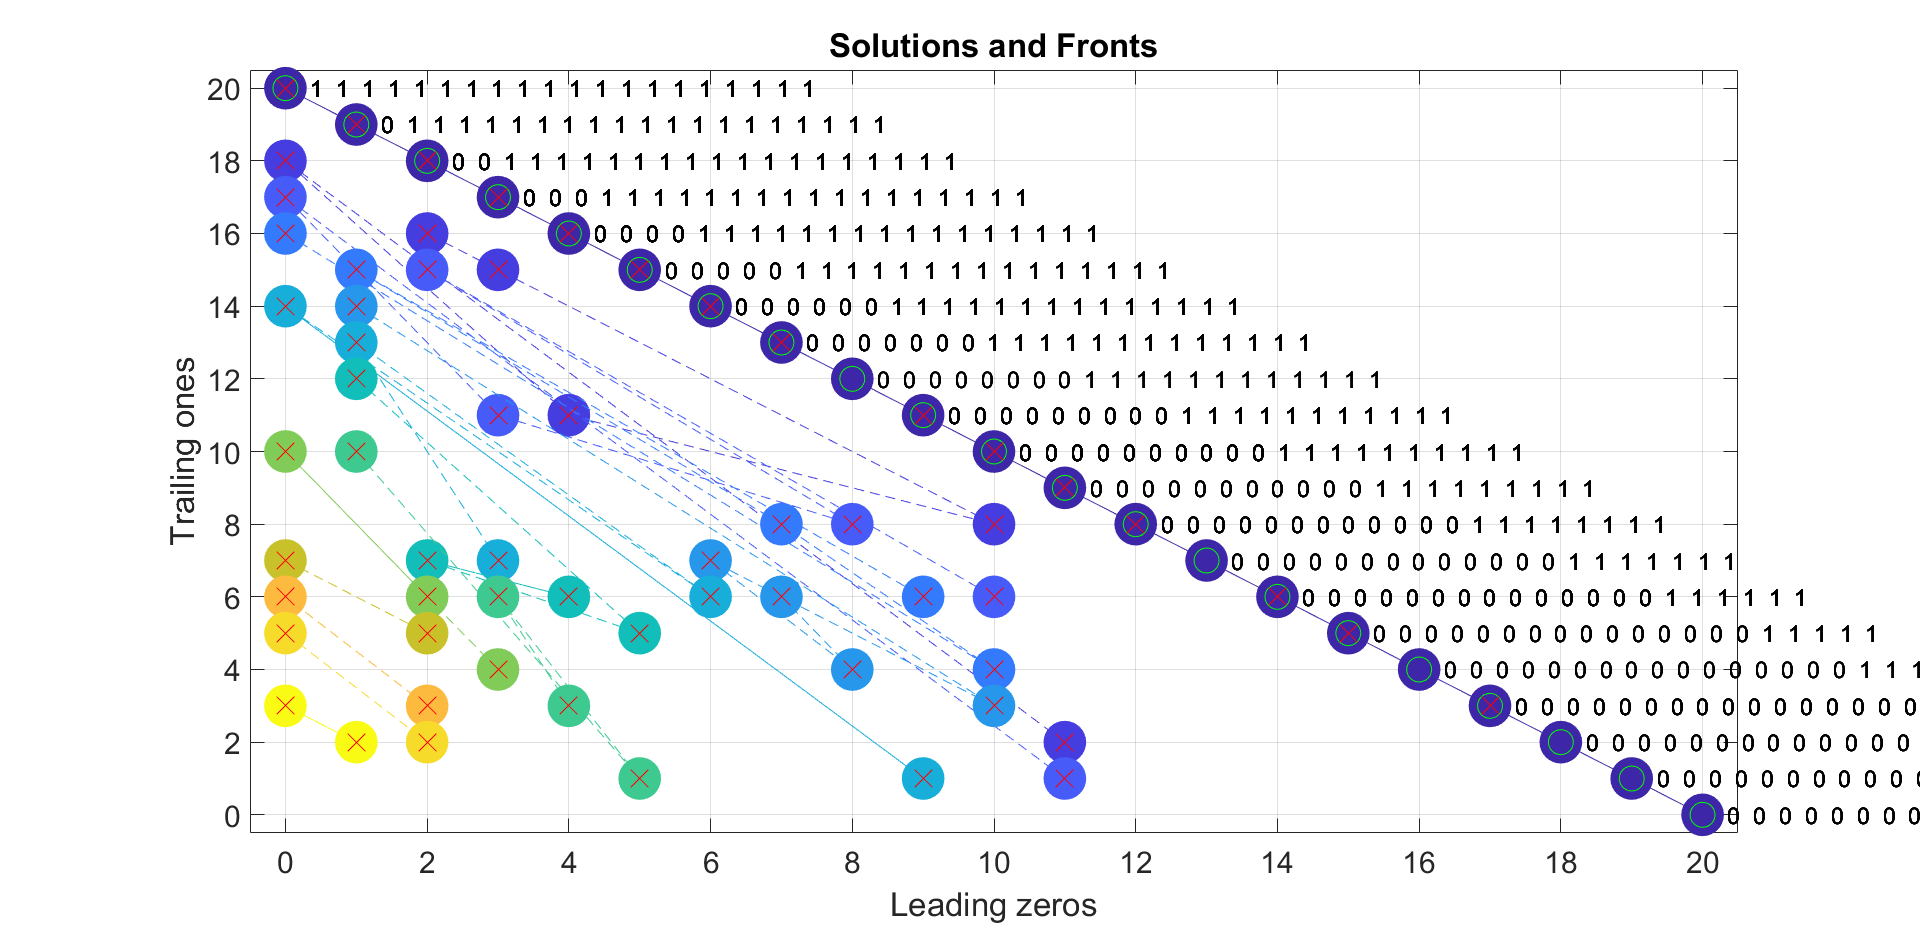
\includegraphics[width=\textwidth]{code/final_plot_100pop100gen}
		\\ plot for 100 generations and 100 population
		\label{finalplot100pop1000gen}
	\end{center}

	\begin{figure}
		\centering
		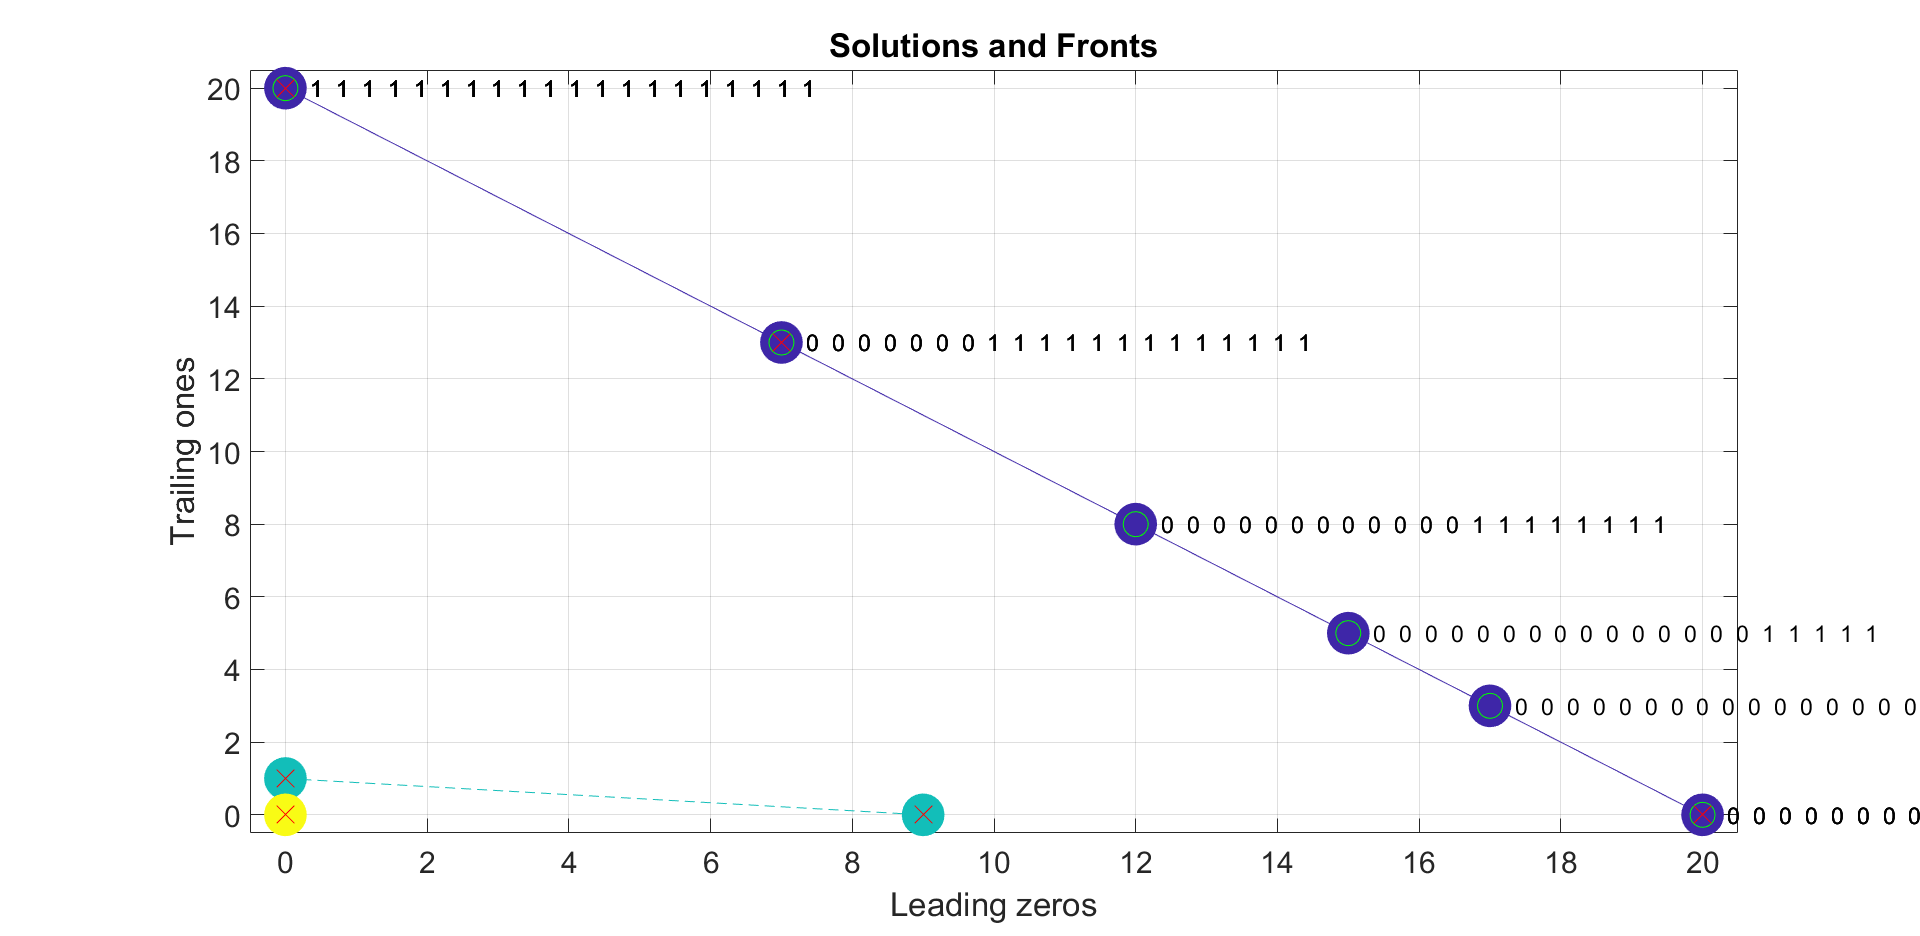
\includegraphics[width=\textwidth]{code/final_plot_10pop1000gen}
		\caption{plot for 1000 generations and 10 population}
		\label{finalplot10pop1000gen}
	\end{figure}
\newpage
	\textbf{ From the above plots it can be appreciated the benefits of having a bigger population size instead of having a higher number of generations. Having more individuals in the populations allows the algorithm to develop the Pareto front much faster than with fewer individuals in the population.}


	\item (5pts) Imagine you were to replace the objective of ``trailing zeros'' with ``largest binary number''. Predict the result, and give your reasoning.\\
	\textbf{ The final plot of the Pareto front would have a positive slope as both fitness increase whenever a new 1 is added. Also, the individual having the maximum fitness for both the leading ones and largest binary number occupying the position 20,20 on the plot and the individual with the least fitness occupying the position 0,0 on the same plot.}
	\item (5pts) Imagine you were to add a third objective: ``non-consecutive ones and zeros'' (ones not touching ones and zeros not touching zeros, e.g. 0101 and 1010 are the most optimal 4 bit solutions). How would you adjust the hyperparameters to get a satisfactory result?\\
	\textbf{The population size and number of generations should be increased accordingly. As it would be required to have more individuals to increase the exploration and with that find the non dominated solutions that conform the Pareto front}
	\item (5pts) In many GAs and ESs populations must be ranked, but no special methods are used. Why is a faster sort in MOO so important?\\
	\textbf{Because the computational complexity is $O(MN^2)$ in the worst case(given a number of fitness functions), thus greatly reducing the run time for these high-dimensional MOO problems.}
\end{itemize}


\newpage
\subsection{** Extra Credit ** (+ 10pts in examination)}
Implement the third objective ``non-consecutive ones and zeros''
\begin{enumerate}
	\item How many non-dominated solutions are possible? (Hint: start with a smaller length and test)\\
	\textbf{We explored the possible solutions for this problem increasing the popSize up to 600 individuals and we found out 115 unique possible solutions with 200 generations. We believe that possibly there could be a few more unique solutions, but we were not able to find them :c. For the sake of an argument we will stay that there could be 120 unique non dominated solutions.}
	\item What changes did you make to the algorithm and hyperparameters to get a good result?\\
	\textbf{ We changed the population size to 600 to increase the exploration and by that find as many unique non dominated solutions as possible.}
	\item List the solutions in your 1st front. Are they all Pareto optimal? How complete is your front (in percentage, based on $\#1$)\\
	\textbf{The list of solutions has been attached as a table at the end of the report. We found 115 possible solutions, which based on our assumption it is 95.83\%.}
	\begin{table}[http]
		\centering
		\caption{My caption}
		\label{my-label}
		\begin{tabular}{|l|}
			\hline
			0     0     1     0     1     0     1     0     1     0     1     0     1     0     1     0     1     0     1     0 \\ \hline
			1     0     1     0     1     0     1     0     1     0     1     1     1     1     1     1     1     1     1     1 \\ \hline
			0     0     0     0     0     0     0     0     0     0     0     0     0     0     0     0     0     0     0     0 \\ \hline
			0     1     0     1     0     1     0     1     0     1     0     1     0     1     0     1     0     1     0     1 \\ \hline
			1     1     1     1     1     1     1     1     1     1     1     1     1     1     1     1     1     1     1     1 \\ \hline
			0     0     0     0     0     0     0     0     0     0     0     1     0     1     0     1     0     1     1     1 \\ \hline
			0     0     0     1     0     1     0     1     0     1     0     1     0     1     1     1     1     1     1     1 \\ \hline
			0     0     0     0     0     0     0     0     0     0     1     0     1     0     1     0     1     0     1     1 \\ \hline
			0     0     0     0     1     0     1     0     1     0     1     0     1     0     1     0     1     1     1     1 \\ \hline
			0     0     0     0     0     0     0     1     0     1     0     1     1     1     1     1     1     1     1     1 \\ \hline
			0     0     0     0     0     1     0     1     1     1     1     1     1     1     1     1     1     1     1     1 \\ \hline
			0     0     0     0     0     0     0     0     0     0     0     0     0     0     1     1     1     1     1     1 \\ \hline
			0     0     0     0     1     0     1     0     1     0     1     0     1     0     1     0     1     0     1     1 \\ \hline
			1     0     1     0     1     1     1     1     1     1     1     1     1     1     1     1     1     1     1     1 \\ \hline
			0     1     0     1     0     1     1     1     1     1     1     1     1     1     1     1     1     1     1     1 \\ \hline
			0     0     1     1     1     1     1     1     1     1     1     1     1     1     1     1     1     1     1     1 \\ \hline
			0     0     0     0     0     0     1     0     1     0     1     0     1     0     1     0     1     0     1     0 \\ \hline
			1     0     1     0     1     0     1     0     1     0     1     0     1     1     1     1     1     1     1     1 \\ \hline
			0     0     0     0     0     0     0     0     0     0     0     0     1     0     1     0     1     0     1     0 \\ \hline
			1     0     1     1     1     1     1     1     1     1     1     1     1     1     1     1     1     1     1     1 \\ \hline
			0     0     0     0     0     0     0     0     0     0     0     0     0     0     0     0     1     0     1     0 \\ \hline
			1     0     1     0     1     0     1     1     1     1     1     1     1     1     1     1     1     1     1     1 \\ \hline
			0     0     0     0     0     0     0     0     0     0     0     0     0     0     1     0     1     0     1     0 \\ \hline
			0     0     0     1     0     1     0     1     0     1     0     1     0     1     0     1     1     1     1     1 \\ \hline
			0     0     1     0     1     0     1     0     1     1     1     1     1     1     1     1     1     1     1     1 \\ \hline
			0     0     1     0     1     0     1     0     1     0     1     1     1     1     1     1     1     1     1     1 \\ \hline
			0     0     0     0     0     0     0     0     0     1     1     1     1     1     1     1     1     1     1     1 \\ \hline
			0     0     0     0     0     0     0     0     0     0     0     0     0     0     0     1     1     1     1     1 \\ \hline
			0     0     0     0     0     0     1     0     1     0     1     0     1     0     1     1     1     1     1     1 \\ \hline
			0     0     0     1     1     1     1     1     1     1     1     1     1     1     1     1     1     1     1     1 \\ \hline
			1     0     1     0     1     0     1     0     1     0     1     0     1     0     1     0     1     1     1     1 \\ \hline
			0     0     0     1     0     1     0     1     0     1     0     1     0     1     0     1     0     1     1     1 \\ \hline
			0     0     1     0     1     0     1     0     1     0     1     0     1     0     1     0     1     0     1     1 \\ \hline
			0     1     0     1     0     1     0     1     0     1     0     1     0     1     0     1     0     1     1     1 \\ \hline
			1     0     1     0     1     0     1     0     1     0     1     0     1     0     1     1     1     1     1     1 \\ \hline
			0     0     0     1     0     1     1     1     1     1     1     1     1     1     1     1     1     1     1     1 \\ \hline
			0     0     0     0     0     0     0     0     1     0     1     1     1     1     1     1     1     1     1     1 \\ \hline
			0     0     0     0     0     0     0     0     0     0     0     0     0     1     1     1     1     1     1     1 \\ \hline
			0     0     0     0     0     0     0     0     0     0     0     0     0     0     0     0     0     0     0     1 \\ \hline
			\end{tabular}
		\end{table}
		\begin{table}[http]
			\centering
			\caption{My caption}
			\label{my-label}
			\begin{tabular}{|l|}
				\hline
			0     0     0     0     0     0     0     0     0     0     0     0     0     0     0     0     0     0     1     0 \\ \hline
			0     0     0     0     0     0     0     0     0     0     0     0     0     0     0     0     0     1     1     1 \\ \hline
			0     1     1     1     1     1     1     1     1     1     1     1     1     1     1     1     1     1     1     1 \\ \hline
			0     0     0     0     0     0     0     0     0     0     0     0     0     1     0     1     1     1     1     1 \\ \hline
			0     1     0     1     0     1     0     1     1     1     1     1     1     1     1     1     1     1     1     1 \\ \hline
			0     0     0     0     0     0     0     0     0     0     0     1     0     1     1     1     1     1     1     1 \\ \hline
			0     0     0     0     0     0     0     0     0     0     1     1     1     1     1     1     1     1     1     1 \\ \hline
			0     0     0     0     0     1     0     1     0     1     0     1     1     1     1     1     1     1     1     1 \\ \hline
			0     0     0     0     0     0     0     0     0     0     0     0     0     0     0     0     1     0     1     1 \\ \hline
			0     0     0     1     0     1     0     1     0     1     0     1     1     1     1     1     1     1     1     1 \\ \hline
			0     0     1     0     1     0     1     1     1     1     1     1     1     1     1     1     1     1     1     1 \\ \hline
			0     0     0     0     1     0     1     0     1     0     1     0     1     0     1     1     1     1     1     1 \\ \hline
			0     0     0     0     0     0     0     0     0     0     1     0     1     0     1     0     1     0     1     0 \\ \hline
			0     0     0     0     0     0     1     0     1     0     1     0     1     0     1     0     1     0     1     1 \\ \hline
			0     0     0     0     1     0     1     0     1     0     1     0     1     0     1     0     1     0     1     0 \\ \hline
			0     0     0     0     0     0     0     1     0     1     0     1     0     1     0     1     1     1     1     1 \\ \hline
			0     0     1     0     1     0     1     0     1     0     1     0     1     0     1     0     1     1     1     1 \\ \hline
			1     0     1     0     1     0     1     0     1     1     1     1     1     1     1     1     1     1     1     1 \\ \hline
			0     0     0     0     0     0     0     0     0     1     0     1     0     1     0     1     0     1     0     1 \\ \hline
			0     0     0     0     1     1     1     1     1     1     1     1     1     1     1     1     1     1     1     1 \\ \hline
			0     0     0     0     0     0     0     0     0     0     0     0     0     1     0     1     0     1     1     1 \\ \hline
			0     1     0     1     1     1     1     1     1     1     1     1     1     1     1     1     1     1     1     1 \\ \hline
			0     0     0     0     0     0     0     0     0     0     0     0     0     0     0     0     0     0     1     1 \\ \hline
			0     0     0     0     0     0     0     0     0     0     0     0     0     0     0     1     0     1     0     1 \\ \hline
			0     0     0     0     0     0     0     1     1     1     1     1     1     1     1     1     1     1     1     1 \\ \hline
			0     0     0     0     0     1     1     1     1     1     1     1     1     1     1     1     1     1     1     1 \\ \hline
			0     1     0     1     0     1     0     1     0     1     0     1     0     1     0     1     1     1     1     1 \\ \hline
			0     1     0     1     0     1     0     1     0     1     0     1     1     1     1     1     1     1     1     1 \\ \hline
			0     0     0     0     0     0     0     0     0     0     0     0     1     1     1     1     1     1     1     1 \\ \hline
			0     0     0     0     0     0     0     0     1     0     1     0     1     1     1     1     1     1     1     1 \\ \hline
			0     0     0     0     0     0     1     0     1     0     1     0     1     0     1     0     1     1     1     1 \\ \hline
			0     0     0     0     1     0     1     1     1     1     1     1     1     1     1     1     1     1     1     1 \\ \hline
			0     0     0     0     0     0     0     0     0     0     1     0     1     0     1     1     1     1     1     1 \\ \hline
			0     0     0     0     0     0     0     0     0     0     0     0     0     0     0     0     1     1     1     1 \\ \hline
			0     0     0     0     0     0     0     0     0     0     0     0     1     0     1     0     1     0     1     1 \\ \hline
			0     0     0     0     0     0     0     0     1     0     1     0     1     0     1     0     1     0     1     0 \\ \hline
			0     0     0     0     0     0     0     1     0     1     1     1     1     1     1     1     1     1     1     1 \\ \hline
			0     0     0     0     0     0     0     0     0     0     0     1     1     1     1     1     1     1     1     1 \\ \hline
		\end{tabular}
	\end{table}
	\begin{table}[http]
		\centering
		\caption{My caption}
		\label{my-label}
		\begin{tabular}{|l|}
			\hline
			0     0     0     0     0     1     0     1     0     1     0     1     0     1     0     1     0     1     0     1 \\ \hline
			0     0     0     0     0     0     0     0     0     1     0     1     0     1     0     1     1     1     1     1 \\ \hline
			0     0     0     0     1     0     1     0     1     1     1     1     1     1     1     1     1     1     1     1 \\ \hline
			0     0     0     0     0     0     0     0     0     0     0     0     1     0     1     1     1     1     1     1 \\ \hline
			0     0     0     0     0     0     0     1     0     1     0     1     0     1     0     1     0     1     1     1 \\ \hline
			0     0     0     0     0     0     0     0     0     0     0     0     0     0     0     1     0     1     1     1 \\ \hline
			0     0     1     0     1     0     1     0     1     0     1     0     1     0     1     1     1     1     1     1 \\ \hline
			0     0     0     0     0     0     0     1     0     1     0     1     0     1     1     1     1     1     1     1 \\ \hline
			0     1     0     1     0     1     0     1     0     1     1     1     1     1     1     1     1     1     1     1 \\ \hline
			0     0     0     0     0     0     0     0     1     0     1     0     1     0     1     1     1     1     1     1 \\ \hline
			0     0     0     0     0     0     0     0     0     0     1     0     1     1     1     1     1     1     1     1 \\ \hline
			0     0     0     0     0     0     0     0     0     0     0     0     0     0     1     0     1     0     1     1 \\ \hline
			0     0     0     0     0     1     0     1     0     1     0     1     0     1     0     1     1     1     1     1 \\ \hline
			0     0     0     0     0     0     0     0     1     1     1     1     1     1     1     1     1     1     1     1 \\ \hline
			0     0     0     0     0     0     1     0     1     1     1     1     1     1     1     1     1     1     1     1 \\ \hline
			0     0     0     0     0     0     0     0     0     1     0     1     0     1     0     1     0     1     1     1 \\ \hline
			0     0     0     0     0     0     0     0     0     0     0     1     0     1     0     1     0     1     0     1 \\ \hline
			0     1     0     1     0     1     0     1     0     1     0     1     0     1     1     1     1     1     1     1 \\ \hline
			1     0     1     0     1     0     1     0     1     0     1     0     1     0     1     0     1     0     1     1 \\ \hline
			0     0     0     1     0     1     0     1     0     1     0     1     0     1     0     1     0     1     0     1 \\ \hline
			0     0     0     0     0     0     0     0     0     1     0     1     0     1     1     1     1     1     1     1 \\ \hline
			0     0     0     0     0     0     0     0     0     0     0     0     0     0     0     0     0     1     0     1 \\ \hline
			0     0     0     0     0     0     0     0     0     0     1     0     1     0     1     0     1     1     1     1 \\ \hline
			0     0     0     0     0     0     0     1     0     1     0     1     0     1     0     1     0     1     0     1 \\ \hline
			0     0     0     0     1     0     1     0     1     0     1     0     1     1     1     1     1     1     1     1 \\ \hline
			0     0     1     0     1     1     1     1     1     1     1     1     1     1     1     1     1     1     1     1 \\ \hline
			0     0     0     0     0     0     0     0     0     1     0     1     1     1     1     1     1     1     1     1 \\ \hline
			0     0     0     0     0     1     0     1     0     1     1     1     1     1     1     1     1     1     1     1 \\ \hline
			0     0     0     0     0     0     1     0     1     0     1     0     1     1     1     1     1     1     1     1 \\ \hline
			0     0     0     0     1     0     1     0     1     0     1     1     1     1     1     1     1     1     1     1 \\ \hline
			0     0     0     0     0     0     0     0     0     0     0     1     0     1     0     1     1     1     1     1 \\ \hline
			0     0     0     0     0     0     1     1     1     1     1     1     1     1     1     1     1     1     1     1 \\ \hline
			0     0     0     1     0     1     0     1     0     1     1     1     1     1     1     1     1     1     1     1 \\ \hline
			0     0     0     0     0     0     0     0     0     0     0     0     0     0     1     0     1     1     1     1 \\ \hline
			0     0     0     0     0     0     0     0     0     0     0     0     0     1     0     1     0     1     0     1 \\ \hline
			0     0     0     0     0     0     0     0     1     0     1     0     1     0     1     0     1     1     1     1 \\ \hline
			0     0     0     1     0     1     0     1     1     1     1     1     1     1     1     1     1     1     1     1 \\ \hline
			0     0     0     0     0     1     0     1     0     1     0     1     0     1     1     1     1     1     1     1 \\ \hline
		\end{tabular}
	\end{table}
	\item Plot the end result in 3D. (Use \mcode{plot3} or \mcode{scatter3})
			\begin{figure}
			\centering
			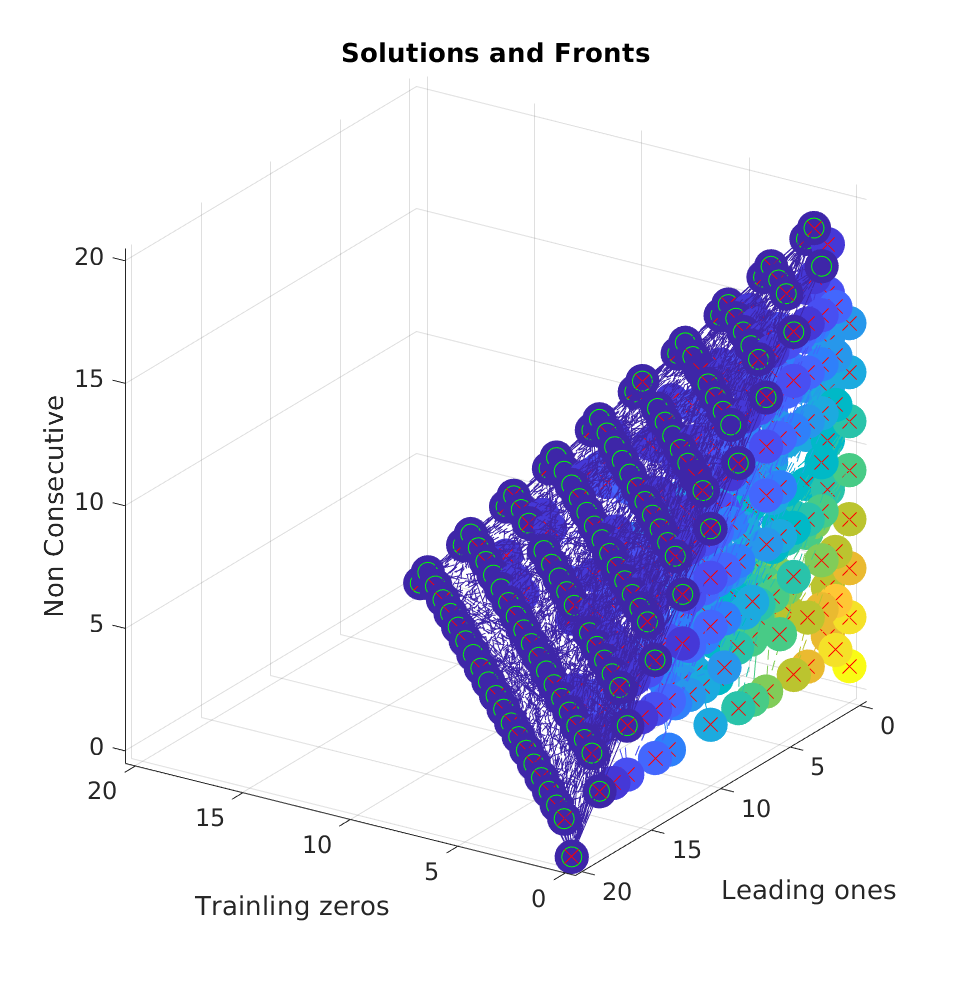
\includegraphics[width=\textwidth]{code/Extra_credit}
			\caption{The plot obtained for non-consecutive zeros and ones with population of 600 and 200 generations.}
			\label{extracredit}
		\end{figure}
\end{enumerate}


\end{document}
